\chapter{Block Codes (Hamming, BCH, Reed-Solomon)}
\label{ch:block-codes}

\begin{nontechnical}
\textbf{Block codes are like adding sudoku-style clues to your message}---if some numbers get corrupted, you can solve for the missing ones using the patterns!

\textbf{Simple idea:}
\begin{itemize}
\item Take a block of data (e.g., 4 bits: \texttt{1011})
\item Add parity bits using math (e.g., 3 extra bits: \texttt{010})
\item Send the whole thing: \texttt{1011010} (7 bits total)
\item Receiver checks if the math works out
\item If errors detected, use the math to FIX them!
\end{itemize}

\textbf{Real uses:} 
\begin{itemize}
\item \textbf{RAM}: Hamming codes fix single-bit errors in computer memory
\item \textbf{QR codes}: Reed-Solomon allows scanning with 30\% damage
\item \textbf{CDs/DVDs}: Reed-Solomon fixes scratches (up to 2.5~mm!)
\item \textbf{Satellite}: Voyager probes use RS codes to send photos from interstellar space
\end{itemize}

\textbf{Trade-off:} More redundancy = fix more errors but less efficient. Hamming (7,4): 43\% overhead, fixes 1 error. Reed-Solomon (255,223): 14\% overhead, fixes 16 symbol errors!
\end{nontechnical}

\section{Overview}

\textbf{Block codes} are a fundamental class of error-correcting codes that encode fixed-length blocks of $k$ data symbols into $n$ code symbols by adding $n-k$ redundant parity symbols.

\begin{keyconcept}
Block codes provide \textbf{guaranteed error correction capability} through systematic redundancy. An $(n,k)$ block code with minimum distance $d_{\min}$ can \textbf{detect} up to $d_{\min}-1$ errors and \textbf{correct} up to $t = \lfloor (d_{\min}-1)/2 \rfloor$ errors.
\end{keyconcept}

The notation $(n,k)$ specifies:
\begin{itemize}
\item $n$ = codeword length (total symbols)
\item $k$ = message length (data symbols)
\item $n-k$ = redundancy (parity symbols)
\end{itemize}

The \textbf{code rate} measures efficiency:
\begin{equation}
R = \frac{k}{n}
\end{equation}
where:
\begin{itemize}
\item $R$ = code rate (dimensionless, $0 < R < 1$)
\item Higher $R$ means more efficient (less redundancy)
\item Lower $R$ means stronger error correction
\end{itemize}

Block codes divide into three main categories:
\begin{enumerate}
\item \textbf{Linear block codes}: Codewords form a vector space; encoding via matrix multiplication
\item \textbf{Cyclic codes}: Cyclic shifts of codewords are also valid codewords (enables shift-register implementation)
\item \textbf{Non-linear codes}: More complex structure (rarely used in practice)
\end{enumerate}

\section{Mathematical Description}

\subsection{Linear Block Codes}

A linear block code over $\mathrm{GF}(q)$ is a $k$-dimensional subspace of the $n$-dimensional vector space $\mathrm{GF}(q)^n$. For binary codes, $q=2$.

\subsection{Generator Matrix}

Encoding in linear block codes uses matrix multiplication:
\begin{equation}
\mathbf{c} = \mathbf{d} \cdot G
\end{equation}
where:
\begin{itemize}
\item $\mathbf{d}$ = data vector $(1 \times k)$
\item $G$ = generator matrix $(k \times n)$
\item $\mathbf{c}$ = codeword vector $(1 \times n)$
\end{itemize}

For \textbf{systematic encoding}, the generator matrix takes the form:
\begin{equation}
G = [I_k \mid P]
\end{equation}
where:
\begin{itemize}
\item $I_k$ = $k \times k$ identity matrix
\item $P$ = $k \times (n-k)$ parity submatrix
\end{itemize}

This produces codewords where the first $k$ symbols are the original data (unchanged), and the last $n-k$ symbols are parity.

\subsection{Parity-Check Matrix}

The parity-check matrix $H$ of dimension $(n-k) \times n$ satisfies:
\begin{equation}
\mathbf{c} \cdot H^T = \mathbf{0}
\end{equation}
for all valid codewords $\mathbf{c}$.

For systematic codes with $G = [I_k \mid P]$, the parity-check matrix is:
\begin{equation}
H = [-P^T \mid I_{n-k}]
\end{equation}
where:
\begin{itemize}
\item $P^T$ = transpose of parity submatrix
\item $I_{n-k}$ = $(n-k) \times (n-k)$ identity matrix
\item For binary codes, $-P^T = P^T$ (modulo-2 arithmetic)
\end{itemize}

\subsection{Syndrome Decoding}

When a codeword $\mathbf{c}$ is transmitted through a noisy channel, the received vector is:
\begin{equation}
\mathbf{r} = \mathbf{c} + \mathbf{e}
\end{equation}
where:
\begin{itemize}
\item $\mathbf{r}$ = received vector
\item $\mathbf{e}$ = error vector (1 where errors occurred, 0 elsewhere)
\end{itemize}

The \textbf{syndrome} is computed as:
\begin{equation}
\mathbf{s} = \mathbf{r} \cdot H^T
\end{equation}

Since $\mathbf{c} \cdot H^T = \mathbf{0}$:
\begin{equation}
\mathbf{s} = (\mathbf{c} + \mathbf{e}) \cdot H^T = \mathbf{e} \cdot H^T
\end{equation}

\textbf{Key property:} The syndrome depends \textbf{only on the error pattern}, not on the transmitted codeword.

\textbf{Decoding procedure:}
\begin{enumerate}
\item Calculate syndrome $\mathbf{s} = \mathbf{r} \cdot H^T$
\item Look up error pattern $\mathbf{e}$ from syndrome table
\item Correct: $\hat{\mathbf{c}} = \mathbf{r} - \mathbf{e}$ (for binary: $\mathbf{r} \oplus \mathbf{e}$)
\end{enumerate}

\subsection{Block Diagram: Encoding and Decoding}

\begin{center}
\begin{tikzpicture}[
  block/.style={rectangle, draw, minimum width=2.5cm, minimum height=1cm, font=\sffamily\small, align=center},
  node distance=2.5cm,
  font=\small
]
% Encoder section
\node (input) {\sffamily Data\\$\mathbf{d}$\\$(k$ bits$)$};
\node[block, right of=input, node distance=3cm] (encoder) {Encoder\\$\mathbf{c}=\mathbf{d}G$};
\node[block, right of=encoder, node distance=3.2cm] (channel) {Noisy\\Channel};
\node[right of=channel, node distance=3cm] (received) {\sffamily Received\\$\mathbf{r}$};

% Decoder section
\node[block, below of=received, node distance=2cm] (syndrome) {Syndrome\\$\mathbf{s}=\mathbf{r}H^T$};
\node[block, left of=syndrome, node distance=3.5cm] (lookup) {Error\\Lookup};
\node[block, left of=lookup, node distance=3.5cm] (correct) {Correct\\$\hat{\mathbf{c}}=\mathbf{r}-\mathbf{e}$};
\node[left of=correct, node distance=3.2cm] (output) {\sffamily Data\\$\hat{\mathbf{d}}$\\$(k$ bits$)$};

% Arrows - Encoder path
\draw[->,thick] (input) -- (encoder);
\draw[->,thick] (encoder) -- node[above,font=\scriptsize] {$\mathbf{c}$ ($n$ bits)} (channel);
\draw[->,thick] (channel) -- node[above,font=\scriptsize] {$+\mathbf{e}$} (received);

% Arrows - Decoder path
\draw[->,thick] (received) -- (syndrome);
\draw[->,thick] (syndrome) -- node[above,font=\scriptsize] {$\mathbf{s}$} (lookup);
\draw[->,thick] (lookup) -- node[above,font=\scriptsize] {$\mathbf{e}$} (correct);
\draw[->,thick] (correct) -- (output);

% Annotations
\node[above=0.3cm of encoder, font=\scriptsize\itshape] {Transmitter};
\node[above=0.3cm of syndrome, font=\scriptsize\itshape] {Receiver};
\end{tikzpicture}
\end{center}

\section{Hamming Codes}\label{hamming-codes}

Hamming codes, invented by Richard Hamming in 1950, form a family of perfect single-error-correcting codes.

\subsection{Parameters and Properties}

The Hamming code family is defined by:
\begin{equation}
(n, k) = (2^m - 1, 2^m - m - 1) \quad \text{for } m \geq 2
\end{equation}
where:
\begin{itemize}
\item $m$ = number of parity bits
\item $n = 2^m - 1$ = codeword length
\item $k = 2^m - m - 1$ = data length
\end{itemize}

Common Hamming codes:
\begin{itemize}
\item $(7, 4)$: 4 data bits, 3 parity bits
\item $(15, 11)$: 11 data bits, 4 parity bits
\item $(31, 26)$: 26 data bits, 5 parity bits
\end{itemize}

The minimum Hamming distance is:
\begin{equation}
d_{\min} = 3
\end{equation}

This provides:
\begin{itemize}
\item \textbf{Error correction:} $t = \lfloor (d_{\min}-1)/2 \rfloor = 1$ bit
\item \textbf{Error detection:} $d_{\min} - 1 = 2$ bits
\end{itemize}

\begin{keyconcept}
Hamming codes are \textbf{perfect codes}---they achieve the Hamming bound with equality. Every possible received vector is within distance 1 of exactly one codeword, meaning the sphere-packing efficiency is 100\%.
\end{keyconcept}

\subsection{Hamming(7,4) Example}\label{hamming74-example}

The Hamming(7,4) code encodes 4 data bits into 7 code bits.

\textbf{Generator matrix} (systematic form):
\begin{equation}
G = \begin{bmatrix}
1 & 0 & 0 & 0 & 1 & 1 & 0 \\
0 & 1 & 0 & 0 & 1 & 0 & 1 \\
0 & 0 & 1 & 0 & 0 & 1 & 1 \\
0 & 0 & 0 & 1 & 1 & 1 & 1
\end{bmatrix} = [I_4 \mid P]
\end{equation}
where:
\begin{itemize}
\item Columns 1--4: Identity matrix (data bits pass through unchanged)
\item Columns 5--7: Parity bits computed from data
\end{itemize}

\textbf{Parity-check matrix}:
\begin{equation}
H = \begin{bmatrix}
1 & 1 & 0 & 1 & 1 & 0 & 0 \\
1 & 0 & 1 & 1 & 0 & 1 & 0 \\
0 & 1 & 1 & 1 & 0 & 0 & 1
\end{bmatrix} = [P^T \mid I_3]
\end{equation}

\subsection{TikZ Diagram: Generator Matrix Structure}

\begin{center}
\begin{tikzpicture}[scale=0.8]
% Draw the matrix
\matrix (m) [matrix of math nodes,
  left delimiter=[,
  right delimiter={]},
  row sep=0.5cm,
  column sep=0.4cm] {
  1 & 0 & 0 & 0 & 1 & 1 & 0 \\
  0 & 1 & 0 & 0 & 1 & 0 & 1 \\
  0 & 0 & 1 & 0 & 0 & 1 & 1 \\
  0 & 0 & 0 & 1 & 1 & 1 & 1 \\
};

% Highlight identity section
\draw[thick, blue] ($(m-1-1.north west) + (-0.15,0.15)$) rectangle ($(m-4-4.south east) + (0.15,-0.15)$);
\node[above=0.3cm of m-1-2, blue, font=\sffamily\small] {$I_4$ (Data)};

% Highlight parity section
\draw[thick, red] ($(m-1-5.north west) + (-0.15,0.15)$) rectangle ($(m-4-7.south east) + (0.15,-0.15)$);
\node[above=0.3cm of m-1-6, red, font=\sffamily\small] {$P$ (Parity)};

% Arrows showing structure
\draw[<->, thick] ($(m-1-1.north west) + (-0.3,0.5)$) -- ($(m-1-4.north east) + (0.3,0.5)$) node[midway, above, font=\scriptsize] {$k=4$ columns};
\draw[<->, thick] ($(m-1-5.north west) + (-0.3,0.5)$) -- ($(m-1-7.north east) + (0.3,0.5)$) node[midway, above, font=\scriptsize] {$n-k=3$ columns};
\end{tikzpicture}
\end{center}

\subsection{Encoding Example}

\textbf{Data vector:} $\mathbf{d} = [1, 0, 1, 1]$

\textbf{Encoding operation:}
\begin{equation}
\mathbf{c} = \mathbf{d} \cdot G = [1, 0, 1, 1] \cdot G = [1, 0, 1, 1, 0, 0, 1]
\end{equation}
where:
\begin{itemize}
\item First 4 bits $[1, 0, 1, 1]$ are the original data (systematic)
\item Last 3 bits $[0, 0, 1]$ are computed parity bits
\end{itemize}

\textbf{Verification using parity-check matrix:}
\begin{equation}
\mathbf{c} \cdot H^T = [0, 0, 0]^T \quad \checkmark
\end{equation}

A zero syndrome confirms this is a valid codeword.

\subsection{Decoding Example with Error Correction}

\textbf{Transmitted codeword:} $\mathbf{c} = [1, 0, 1, 1, 0, 0, 1]$

\textbf{Received vector (with error in position 4):} 
\begin{equation}
\mathbf{r} = [1, 0, 1, \underline{0}, 0, 0, 1]
\end{equation}

\textbf{Syndrome calculation:}
\begin{equation}
\mathbf{s} = \mathbf{r} \cdot H^T = [1, 1, 1]^T
\end{equation}

\textbf{Error localization:} The syndrome $[1, 1, 1]^T$ matches column 4 of $H$, indicating the error is in bit position 4.

\textbf{Correction:}
\begin{equation}
\hat{\mathbf{c}} = \mathbf{r} \oplus \mathbf{e} = [1, 0, 1, 0, 0, 0, 1] \oplus [0, 0, 0, 1, 0, 0, 0] = [1, 0, 1, 1, 0, 0, 1]
\end{equation}
where:
\begin{itemize}
\item $\mathbf{e} = [0, 0, 0, 1, 0, 0, 0]$ is the error vector
\item $\oplus$ denotes XOR (modulo-2 addition)
\end{itemize}

\begin{calloutbox}{Syndrome Decoding Insight}
The syndrome uniquely identifies the error position. For Hamming codes, the syndrome value equals the binary representation of the error position, making decoding extremely efficient.
\end{calloutbox}

\subsection{Extended Hamming Code}

Adding one overall parity bit to a Hamming code creates an \textbf{extended Hamming code}:
\begin{equation}
(n, k) = (2^m, 2^m - m - 1)
\end{equation}

This increases the minimum distance:
\begin{equation}
d_{\min} = 4
\end{equation}

\textbf{Capabilities:}
\begin{itemize}
\item \textbf{Correct:} 1 error ($t = 1$)
\item \textbf{Detect:} 3 errors
\item Known as \textbf{SECDED}: Single Error Correction, Double Error Detection
\end{itemize}

\textbf{Example:} Hamming(8,4) with $d_{\min} = 4$ is used in ECC RAM to protect against single-bit upsets while detecting multi-bit errors.

\section{BCH Codes}\label{bch-codes}

\textbf{Bose-Chaudhuri-Hocquenghem (BCH) codes} are a class of powerful cyclic codes that generalize Hamming codes to correct multiple errors.

\subsection{BCH Code Parameters}

BCH codes over $\mathrm{GF}(q)$ are characterized by:
\begin{equation}
(n, k, d_{\min})
\end{equation}
where:
\begin{itemize}
\item $n$ = codeword length
\item $k$ = message length
\item $d_{\min}$ = minimum distance
\end{itemize}

\textbf{Key feature:} BCH codes can be \textbf{designed for any desired error correction capability} $t$ by choosing appropriate parameters.

\subsection{Binary BCH Code Properties}

For binary BCH codes ($q = 2$):

\textbf{Block length:}
\begin{equation}
n = 2^m - 1 \quad \text{for } m \geq 3
\end{equation}

\textbf{Minimum distance guarantee:}
\begin{equation}
d_{\min} \geq 2t + 1
\end{equation}
where:
\begin{itemize}
\item $t$ = designed error correction capability (number of errors correctable)
\item This guarantees correction of $t$ errors
\end{itemize}

\textbf{Generator polynomial:} BCH codes are defined by their generator polynomial $g(x)$ of degree $n-k$:
\begin{equation}
g(x) = \mathrm{LCM}(m_1(x), m_2(x), \ldots, m_{2t}(x))
\end{equation}
where $m_i(x)$ are the minimal polynomials of $\alpha^i$ over $\mathrm{GF}(2^m)$.

\textbf{Decoding algorithms:}
\begin{itemize}
\item Berlekamp-Massey algorithm (efficient for multiple errors)
\item Peterson-Gorenstein-Zierler algorithm
\item Euclidean algorithm
\end{itemize}

\subsubsection{Common BCH Codes}\label{common-bch-codes}

{\def\LTcaptype{} % do not increment counter
\begin{longtable}[]{@{}lllll@{}}
\toprule\noalign{}
Code & \((n, k)\) & \(t\) & \(d_{\min}\) & Rate \\
\midrule\noalign{}
\endhead
\bottomrule\noalign{}
\endlastfoot
\textbf{BCH(15,11)} & (15, 11) & 1 & 3 & 0.73 \\
\textbf{BCH(15,7)} & (15, 7) & 2 & 5 & 0.47 \\
\textbf{BCH(31,26)} & (31, 26) & 1 & 3 & 0.84 \\
\textbf{BCH(31,21)} & (31, 21) & 2 & 5 & 0.68 \\
\textbf{BCH(31,16)} & (31, 16) & 3 & 7 & 0.52 \\
\textbf{BCH(63,51)} & (63, 51) & 2 & 5 & 0.81 \\
\textbf{BCH(127,106)} & (127, 106) & 3 & 7 & 0.83 \\
\end{longtable}
}

\begin{center}\rule{0.5\linewidth}{0.5pt}\end{center}

\subsubsection{BCH vs Hamming}\label{bch-vs-hamming}

\textbf{Hamming codes}: Special case of BCH (\(t = 1\))

\textbf{BCH advantage}: Design for any \(t\) (multiple error correction)

\textbf{Example}: BCH(31,16,7) - Corrects \(t = 3\) errors -
Hamming(31,26,3) corrects only \(t = 1\)

\begin{center}\rule{0.5\linewidth}{0.5pt}\end{center}

\section{Reed-Solomon Codes}\label{reed-solomon-codes}

\textbf{Reed-Solomon (RS) codes} are non-binary BCH codes operating over Galois fields $\mathrm{GF}(2^m)$. They are among the most widely used error-correcting codes due to their excellent burst error correction capability.

\subsection{RS Code Parameters}

An RS code over $\mathrm{GF}(2^m)$ is denoted RS$(n,k)$:
\begin{equation}
n = 2^m - 1 \quad \text{(maximum block length)}
\end{equation}
where:
\begin{itemize}
\item $n$ = codeword length (in $m$-bit symbols)
\item $k$ = message length (in $m$-bit symbols)
\item $m$ = bits per symbol (typically $m = 8$ for byte-oriented systems)
\end{itemize}

\textbf{Number of parity symbols:}
\begin{equation}
n - k = 2t
\end{equation}
where:
\begin{itemize}
\item $t$ = number of symbol errors that can be corrected
\end{itemize}

\subsection{Maximum Distance Separable Property}

RS codes are \textbf{Maximum Distance Separable (MDS)}, meaning they achieve the Singleton bound:
\begin{equation}
d_{\min} = n - k + 1
\end{equation}
where:
\begin{itemize}
\item $d_{\min}$ = minimum distance (in symbols)
\item This is the maximum possible for any code with given $n$ and $k$
\end{itemize}

\textbf{Error correction capability:}
\begin{equation}
t = \left\lfloor \frac{d_{\min} - 1}{2} \right\rfloor = \left\lfloor \frac{n-k}{2} \right\rfloor
\end{equation}

\begin{keyconcept}
The MDS property makes RS codes \textbf{optimal}---no other $(n,k)$ code can correct more errors. This explains their dominance in applications requiring maximum error correction for a given redundancy level.
\end{keyconcept}

\subsection{RS Code Advantages}

\begin{enumerate}
\item \textbf{Burst error correction}: One symbol error can contain up to $m$ bit errors, making RS codes ideal for channels with burst noise
\item \textbf{Optimal distance}: MDS property ensures maximum error correction for given redundancy
\item \textbf{Well-understood decoding}: Efficient algorithms (Berlekamp-Massey, Euclidean)
\item \textbf{Flexible}: Can be shortened or punctured for different rates
\item \textbf{Widely deployed}: Proven track record in CDs, DVDs, QR codes, satellites
\end{enumerate}

\subsubsection{Common Reed-Solomon
Codes}\label{common-reed-solomon-codes}

{\def\LTcaptype{} % do not increment counter
\begin{longtable}[]{@{}
  >{\raggedright\arraybackslash}p{(\linewidth - 10\tabcolsep) * \real{0.2653}}
  >{\raggedright\arraybackslash}p{(\linewidth - 10\tabcolsep) * \real{0.1224}}
  >{\raggedright\arraybackslash}p{(\linewidth - 10\tabcolsep) * \real{0.1020}}
  >{\raggedright\arraybackslash}p{(\linewidth - 10\tabcolsep) * \real{0.2041}}
  >{\raggedright\arraybackslash}p{(\linewidth - 10\tabcolsep) * \real{0.1020}}
  >{\raggedright\arraybackslash}p{(\linewidth - 10\tabcolsep) * \real{0.2041}}@{}}
\toprule\noalign{}
\begin{minipage}[b]{\linewidth}\raggedright
Application
\end{minipage} & \begin{minipage}[b]{\linewidth}\raggedright
Code
\end{minipage} & \begin{minipage}[b]{\linewidth}\raggedright
\(m\)
\end{minipage} & \begin{minipage}[b]{\linewidth}\raggedright
\((n, k)\)
\end{minipage} & \begin{minipage}[b]{\linewidth}\raggedright
\(t\)
\end{minipage} & \begin{minipage}[b]{\linewidth}\raggedright
Overhead
\end{minipage} \\
\midrule\noalign{}
\endhead
\bottomrule\noalign{}
\endlastfoot
\textbf{CD/DVD} & RS(32,28) & 8 & (255,251) shortened & 2 & 14\% \\
\textbf{QR Code} & RS(255,223) & 8 & (255,223) & 16 & 14\% \\
\textbf{DVB (satellite)} & RS(204,188) & 8 & (255,239) shortened & 8 &
8.5\% \\
\textbf{RAID-6} & RS(n, n-2) & 8 & Variable & 2 & 2 disks \\
\textbf{Voyager} & RS(255,223) & 8 & (255,223) & 16 & 14\% \\
\textbf{DSL (ADSL2+)} & RS(255,239) & 8 & (255,239) & 8 & 6.7\% \\
\end{longtable}
}

\begin{center}\rule{0.5\linewidth}{0.5pt}\end{center}

\subsection{Example: QR Code RS(255,223)}

QR codes use RS(255,223) with the following parameters:
\begin{itemize}
\item $m = 8$ (8-bit symbols = bytes)
\item $n = 255$ bytes (codeword length)
\item $k = 223$ bytes (data)
\item $2t = 32$ bytes (parity symbols)
\end{itemize}

\textbf{Error correction capability:}
\begin{equation}
t = \frac{n-k}{2} = \frac{32}{2} = 16 \text{ byte errors}
\end{equation}

\textbf{Burst error tolerance:} If 128 consecutive bits (16 bytes) are corrupted, the code can fully correct them! This is why QR codes work even when partially obscured.

\subsection{RS Encoding}

RS codes use polynomial representation over $\mathrm{GF}(2^m)$.

\textbf{Data polynomial:}
\begin{equation}
D(x) = d_0 + d_1 x + \cdots + d_{k-1} x^{k-1}
\end{equation}
where $d_i \in \mathrm{GF}(2^m)$ are the data symbols.

\textbf{Generator polynomial} (degree $2t = n-k$):
\begin{equation}
g(x) = \prod_{i=1}^{2t} (x - \alpha^i)
\end{equation}
where:
\begin{itemize}
\item $\alpha$ = primitive element of $\mathrm{GF}(2^m)$
\item $\alpha^i$ are the roots of the generator polynomial
\end{itemize}

\textbf{Systematic encoding:}
\begin{equation}
C(x) = x^{2t} D(x) + R(x)
\end{equation}
where:
\begin{itemize}
\item $R(x) = [x^{2t} D(x)] \mod g(x)$ is the parity polynomial
\item Multiplication by $x^{2t}$ shifts data to high-order positions
\end{itemize}

\subsection{RS Decoding}

The RS decoding process consists of five steps:

\textbf{Step 1: Syndrome calculation}
\begin{equation}
S_i = R(\alpha^i) \quad \text{for } i = 1, 2, \ldots, 2t
\end{equation}
where $R(x)$ is the received polynomial.

\textbf{Step 2: Error locator polynomial} computed using Berlekamp-Massey algorithm:
\begin{equation}
\Lambda(x) = 1 + \Lambda_1 x + \Lambda_2 x^2 + \cdots + \Lambda_v x^v
\end{equation}
where $v \leq t$ is the number of errors.

\textbf{Step 3: Error positions} found using Chien search (finding roots of $\Lambda(x)$)

\textbf{Step 4: Error values} computed using Forney algorithm

\textbf{Step 5: Correction}
\begin{equation}
\hat{C}(x) = R(x) - E(x)
\end{equation}
where $E(x)$ is the error polynomial.

\textbf{Computational complexity:}
\begin{itemize}
\item Standard algorithms: $O(t^2)$
\item FFT-based methods: $O(t \log^2 t)$
\end{itemize}

\subsection{TikZ Diagram: Syndrome Decoding Flowchart}

\begin{center}
\begin{tikzpicture}[
  block/.style={rectangle, draw, minimum width=3cm, minimum height=0.8cm, font=\sffamily\small, align=center},
  decision/.style={diamond, draw, minimum width=2.5cm, minimum height=2cm, font=\sffamily\small, align=center, aspect=2},
  node distance=1.8cm,
  font=\small
]
\node[block] (input) {Received $\mathbf{r}$};
\node[block, below of=input] (syndrome) {Calculate Syndrome\\$\mathbf{s} = \mathbf{r} H^T$};
\node[decision, below of=syndrome, node distance=2.5cm] (check) {$\mathbf{s} = 0$?};
\node[block, right of=check, node distance=4cm] (noerror) {No errors\\Output $\mathbf{r}$};
\node[block, below of=check, node distance=2.5cm] (locate) {Locate error\\from syndrome};
\node[block, below of=locate] (correct) {Correct errors\\$\hat{\mathbf{c}} = \mathbf{r} - \mathbf{e}$};
\node[block, below of=correct] (output) {Output $\hat{\mathbf{c}}$};

\draw[->,thick] (input) -- (syndrome);
\draw[->,thick] (syndrome) -- (check);
\draw[->,thick] (check) -- node[above,font=\scriptsize] {Yes} (noerror);
\draw[->,thick] (check) -- node[right,font=\scriptsize] {No} (locate);
\draw[->,thick] (locate) -- (correct);
\draw[->,thick] (correct) -- (output);
\end{tikzpicture}
\end{center}

\section{Performance Analysis}\label{performance-analysis}

\subsection{Error Correction Probability}

For a binary symmetric channel (BSC) with bit error probability $p$, and a code that corrects $t$ errors:

\textbf{Probability of successful decoding:}
\begin{equation}
P_{\text{correct}} = \sum_{i=0}^{t} \binom{n}{i} p^i (1-p)^{n-i}
\end{equation}
where:
\begin{itemize}
\item $\binom{n}{i}$ = number of ways to have $i$ errors in $n$ bits
\item $p^i$ = probability of $i$ errors
\item $(1-p)^{n-i}$ = probability of $n-i$ correct bits
\end{itemize}

\textbf{Block error rate (decoding failure):}
\begin{equation}
P_{\text{block}} = 1 - P_{\text{correct}} = \sum_{i=t+1}^{n} \binom{n}{i} p^i (1-p)^{n-i}
\end{equation}

\subsection{Bit Error Rate Performance}

\textbf{Uncoded BER} on BSC:
\begin{equation}
\text{BER}_{\text{uncoded}} = p
\end{equation}

\textbf{Coded BER} (after decoding):
\begin{equation}
\text{BER}_{\text{coded}} \approx \frac{P_{\text{block}}}{n}
\end{equation}

This approximation assumes errors are uniformly distributed when decoding fails.

\subsection{Example: Hamming(7,4) Performance}

\textbf{Channel:} BSC with $p = 10^{-3}$ (raw BER)

\textbf{Error correction capability:} $t = 1$ error

\textbf{Probability of successful decoding:}
\begin{equation}
\begin{aligned}
P_{\text{correct}} &= (1-p)^7 + \binom{7}{1} p (1-p)^6 \\
&= (0.999)^7 + 7(0.001)(0.999)^6 \\
&= 0.9930 + 0.0069 = 0.9999
\end{aligned}
\end{equation}

\textbf{Block error rate:}
\begin{equation}
P_{\text{block}} = 1 - 0.9999 = 10^{-4}
\end{equation}

\textbf{Coded BER:}
\begin{equation}
\text{BER}_{\text{coded}} \approx \frac{10^{-4}}{7} = 1.4 \times 10^{-5}
\end{equation}

\textbf{Coding gain:}
\begin{equation}
\text{Improvement} = \frac{10^{-3}}{1.4 \times 10^{-5}} \approx 71\times
\end{equation}

\begin{calloutbox}{Performance Improvement}
The Hamming(7,4) code reduces BER from $10^{-3}$ to $1.4 \times 10^{-5}$---a \textbf{71-fold improvement}---with only 75\% overhead (3 parity bits for 4 data bits).
\end{calloutbox}

\subsection{TikZ Diagram: BER Performance Comparison}

\begin{center}
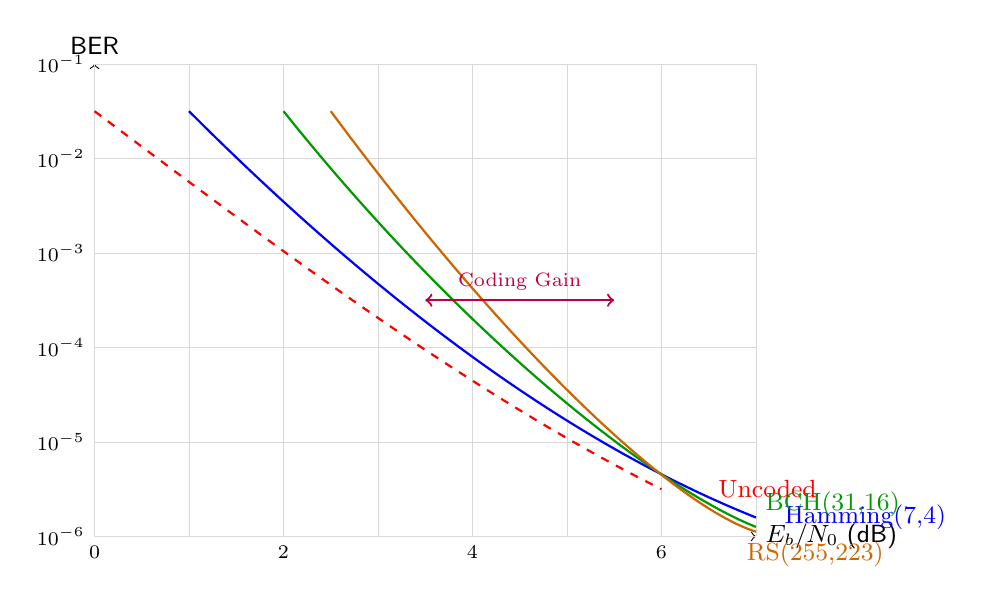
\begin{tikzpicture}[scale=1.2]
% Axes
\draw[->] (0,0) -- (7,0) node[right,font=\sffamily\small] {$E_b/N_0$ (dB)};
\draw[->] (0,0) -- (0,5) node[above,font=\sffamily\small] {BER};

% Grid
\draw[very thin,gray!30] (0,0) grid (7,5);

% Y-axis labels (log scale)
\node[left,font=\scriptsize] at (0,5) {$10^{-1}$};
\node[left,font=\scriptsize] at (0,4) {$10^{-2}$};
\node[left,font=\scriptsize] at (0,3) {$10^{-3}$};
\node[left,font=\scriptsize] at (0,2) {$10^{-4}$};
\node[left,font=\scriptsize] at (0,1) {$10^{-5}$};
\node[left,font=\scriptsize] at (0,0) {$10^{-6}$};

% X-axis labels
\foreach \x in {0,2,4,6}
  \node[below,font=\scriptsize] at (\x,0) {\x};

% Uncoded curve (steeper)
\draw[thick,red,dashed] (0,4.5) .. controls (2,3) and (4,1.5) .. (6,0.5);
\node[red,font=\small,right] at (6.5,0.5) {Uncoded};

% Hamming(7,4) curve
\draw[thick,blue] (1,4.5) .. controls (3,2.5) and (5,1) .. (7,0.2);
\node[blue,font=\small,right] at (7.2,0.2) {Hamming(7,4)};

% BCH(31,16) curve
\draw[thick,green!60!black] (2,4.5) .. controls (4,2) and (6,0.5) .. (7,0.1);
\node[green!60!black,font=\small,above right] at (7,0.1) {BCH(31,16)};

% RS(255,223) curve
\draw[thick,orange!80!black] (2.5,4.5) .. controls (4.5,1.8) and (6.2,0.3) .. (7,0.05);
\node[orange!80!black,font=\small,below right] at (6.8,0.05) {RS(255,223)};

% Annotation: Coding Gain
\draw[<->,thick,purple] (3.5,2.5) -- (5.5,2.5);
\node[purple,font=\scriptsize,above] at (4.5,2.5) {Coding Gain};
\end{tikzpicture}
\end{center}

\textbf{Key observations:}
\begin{itemize}
\item Stronger codes (lower rate) provide steeper BER curves
\item Coding gain increases with $E_b/N_0$
\item At high SNR, powerful codes (RS, BCH) significantly outperform weak codes
\item Trade-off: Stronger codes have lower rate (more overhead)
\end{itemize}

\section{Concatenated Codes}\label{concatenated-codes}

Concatenated codes combine two codes in series to achieve extremely low error rates.

\subsection{Architecture}

\textbf{Outer code:} Strong, symbol-based code (typically Reed-Solomon)
\begin{itemize}
\item Operates on symbols
\item High error correction capability
\item More complex decoding
\end{itemize}

\textbf{Inner code:} Faster, bit-level code (typically convolutional or LDPC)
\begin{itemize}
\item Operates on bits
\item Reduces bit errors to symbol errors
\item Simpler, faster decoding
\end{itemize}

\textbf{Overall code rate:}
\begin{equation}
R_{\text{total}} = R_{\text{inner}} \times R_{\text{outer}}
\end{equation}

\subsection{Example: Voyager Deep Space Mission}

The Voyager spacecraft use concatenated coding for reliable communication from interstellar distances.

\textbf{Inner code:} Convolutional code, rate $R_{\text{inner}} = 1/2$
\begin{itemize}
\item Reduces raw BER from $5 \times 10^{-3}$ to $10^{-5}$
\item Constraint length $K = 7$
\item Viterbi decoding
\end{itemize}

\textbf{Outer code:} RS(255,223), rate $R_{\text{outer}} = 223/255 = 0.875$
\begin{itemize}
\item Corrects up to $t = 16$ symbol (byte) errors
\item At inner code output BER of $10^{-5}$, expected symbol errors are well within correction capability
\item Final BER after RS decoding: $< 10^{-10}$
\end{itemize}

\textbf{Overall system:}
\begin{equation}
R_{\text{total}} = 0.5 \times 0.875 = 0.4375 \quad (56\% \text{ overhead})
\end{equation}

\begin{keyconcept}
Concatenation achieves \textbf{BER improvement from $5 \times 10^{-3}$ to $< 10^{-10}$}---a factor of $5 \times 10^{7}$ improvement---enabling reliable communication from billions of kilometers away.
\end{keyconcept}

\section{Worked Example: Designing a Storage System}

\textbf{Problem:} Design an error correction system for a storage device that experiences random bit errors.

\subsection*{Given Parameters}

\begin{tabular}{@{}ll@{}}
Storage medium BER & $p = 10^{-4}$ \\
Data block size & 512 bytes = 4096 bits \\
Required final BER & $< 10^{-12}$ \\
Maximum overhead & 25\% \\
\end{tabular}

\subsection*{Required}

Select appropriate block code(s) and verify performance.

\subsection*{Solution}

\textit{Step 1: Evaluate single-code options}

For a single Hamming(7,4) code applied to 4096 bits:
\begin{equation}
\text{Blocks needed} = \frac{4096}{4} = 1024 \text{ blocks}
\end{equation}

\begin{equation}
\text{Overhead} = \frac{3}{4} = 75\% \quad \text{(exceeds 25\% limit)}
\end{equation}

Hamming codes alone are unsuitable due to excessive overhead.

\textit{Step 2: Consider Reed-Solomon code}

Use RS(255,223) over $\mathrm{GF}(2^8)$:
\begin{itemize}
\item Each symbol = 8 bits
\item $n = 255$ bytes, $k = 223$ bytes
\item Overhead: $(255-223)/223 = 14.3\%$ \checkmark
\end{itemize}

Number of RS blocks needed:
\begin{equation}
\text{Blocks} = \frac{512 \text{ bytes}}{223 \text{ bytes/block}} \approx 2.3 \text{ blocks}
\end{equation}

Use 3 blocks (with shortened codes).

\textit{Step 3: Calculate expected errors per RS block}

At BER $= 10^{-4}$:
\begin{equation}
\text{Expected bit errors per block} = 255 \times 8 \times 10^{-4} = 0.204 \text{ bits}
\end{equation}

Expected symbol errors (pessimistic, assuming each bit error affects different symbol):
\begin{equation}
\text{Expected symbol errors} \approx 0.204 \text{ symbols}
\end{equation}

Since RS(255,223) corrects up to $t = 16$ symbol errors, this is well within capability.

\textit{Step 4: Calculate block error rate}

Probability that more than 16 symbols have errors (using Poisson approximation with $\lambda = 0.204$):
\begin{equation}
P_{\text{block}} \approx e^{-\lambda} \frac{\lambda^{17}}{17!} + \ldots \approx 10^{-28}
\end{equation}

This is negligible.

\textit{Step 5: Estimate final BER}

\begin{equation}
\text{BER}_{\text{final}} \approx \frac{P_{\text{block}}}{255 \times 8} < 10^{-30}
\end{equation}

\subsection*{Answer}

Use \textbf{RS(255,223)} code with the following characteristics:
\begin{itemize}
\item Overhead: 14.3\% (within 25\% budget)
\item Expected final BER: $< 10^{-30}$ (far exceeds requirement of $10^{-12}$)
\item Number of blocks: 3 (with shortened RS for exact fit)
\end{itemize}

\subsection*{Interpretation}

The RS(255,223) code provides enormous margin over the requirement. In practice, a weaker code like RS(255,239) with only 6.7\% overhead would still meet the $10^{-12}$ requirement while reducing overhead further.

\begin{calloutbox}{Design Lesson}
Reed-Solomon codes are extremely efficient for storage applications. Even with modest overhead (14\%), they can reduce BER by many orders of magnitude, making them ideal for flash memory, hard drives, and optical media.
\end{calloutbox}

\section{Shortened \& Punctured Codes}\label{shortened-punctured-codes}

\subsubsection{Shortened Codes}\label{shortened-codes}

\textbf{Remove \(s\) data symbols} (set to 0, don\textquotesingle t
transmit)

\textbf{Example}: RS(255,223) \$\textbackslash rightarrow\$ RS(204,188)
(DVB) - Set first 51 symbols to 0 - Transmit 204 symbols (188 data + 16
parity) - Same \(d_{\min}\), same correction capability

\begin{center}\rule{0.5\linewidth}{0.5pt}\end{center}

\subsubsection{Punctured Codes}\label{punctured-codes}

\textbf{Delete some parity bits} (increase code rate)

\textbf{Example}: BCH(31,21,5) \$\textbackslash rightarrow\$
BCH(30,21,4) - Remove 1 parity bit - \(d_{\min}\) reduces: 5
\$\textbackslash rightarrow\$ 4 - Correct 2 errors
\$\textbackslash rightarrow\$ 1 error

\textbf{Use case}: Fine-tune code rate for specific channel

\begin{center}\rule{0.5\linewidth}{0.5pt}\end{center}

\section{Applications}\label{applications}

Block codes are deployed in virtually every digital communication and storage system. This section examines key real-world implementations.

\subsection{Computer Memory (ECC DRAM)}

\textbf{System:} Error-Correcting Code (ECC) memory modules

\textbf{Code:} Extended Hamming SECDED (Single Error Correction, Double Error Detection)
\begin{itemize}
\item Configuration: 72 bits total (64 data + 8 parity)
\item Code: Hamming(72,64) with SECDED
\item Corrects: 1-bit errors
\item Detects: 2-bit errors
\end{itemize}

\textbf{Why it matters:} Cosmic rays and alpha particles cause random bit flips in DRAM. ECC prevents system crashes and data corruption, critical for servers and workstations.

\textbf{Advanced systems (Chipkill):} Use Reed-Solomon codes across multiple memory chips to tolerate entire chip failures.

\subsection{Solid-State Drives (Flash Memory)}

\textbf{System:} NAND flash SSDs

\textbf{Code:} BCH codes (traditional) or LDPC (modern)
\begin{itemize}
\item BCH: 10--60 bit correction per 1~KB page
\item Error rate increases with flash wear (P/E cycles)
\item Stronger codes needed for MLC/TLC/QLC flash
\end{itemize}

\textbf{Challenge:} Flash memory error rate increases exponentially with write/erase cycles. Block codes extend device lifetime by correcting errors from cell wear-out.

\subsection{Optical Media (CD/DVD/Blu-ray)}

\textbf{Compact Disc (CD):}
\begin{itemize}
\item Code: CIRC (Cross-Interleaved Reed-Solomon Code)
\item Structure: RS(32,28) outer + RS(28,24) inner with interleaving
\item Capability: Corrects 4000 consecutive error bits ($\sim$2.5~mm scratch)
\item Interleaving spreads burst errors across multiple codewords
\end{itemize}

\textbf{DVD:}
\begin{itemize}
\item Code: RS(208,192)
\item Corrects: 8 symbol errors per block
\item Improved over CD due to higher data density
\end{itemize}

\textbf{Blu-ray:}
\begin{itemize}
\item Code: RS(216,192) or LDPC
\item Higher density requires stronger codes
\end{itemize}

\subsection{QR Codes (2D Barcodes)}

\textbf{System:} Quick Response codes for data encoding

\textbf{Code:} Reed-Solomon with selectable error correction levels

\textbf{Four levels:}
\begin{center}
\begin{tabular}{@{}lll@{}}
\toprule
Level & Recovery & Description \\
\midrule
L & 7\% & Low (default) \\
M & 15\% & Medium \\
Q & 25\% & Quartile \\
H & 30\% & High \\
\bottomrule
\end{tabular}
\end{center}

\textbf{Example (Level H):} QR code can be 30\% obscured (dirt, damage, logos) and still scan successfully. This enables creative QR code designs with embedded graphics.

\subsection{Deep Space Communications}

\textbf{System:} Voyager 1 and 2 spacecraft (launched 1977)

\textbf{Code:} Concatenated coding
\begin{itemize}
\item Inner: Convolutional code, rate 1/2, $K=7$
\item Outer: RS(255,223), corrects 16 byte errors
\item Combined rate: 0.4375 (43.75\% overhead)
\end{itemize}

\textbf{Performance:}
\begin{itemize}
\item Input BER: $5 \times 10^{-3}$ (extremely noisy channel)
\item Output BER: $< 10^{-10}$ (virtually error-free)
\item Improvement: Factor of $5 \times 10^{7}$
\end{itemize}

\textbf{Why critical:} At 24 billion km distance, received signal power is only $-196$~dBm. Without powerful error correction, no communication would be possible.

\subsection{RAID Storage Arrays}

\textbf{System:} RAID-6 disk arrays

\textbf{Code:} Reed-Solomon RS$(n, n-2)$
\begin{itemize}
\item Example: 10 disks (8 data + 2 parity)
\item Tolerates: Any 2 simultaneous disk failures
\item Each disk failure = complete symbol loss
\end{itemize}

\textbf{Advantage:} Dual parity provides better protection than RAID-5 during disk rebuilds, when system is vulnerable.

\subsection{Digital Video Broadcasting (DVB-S2)}

\textbf{System:} Satellite television transmission

\textbf{Code:} Concatenated BCH + LDPC
\begin{itemize}
\item Outer: BCH code
\item Inner: LDPC codes with rates 1/4 to 9/10
\item Adaptive coding based on channel conditions
\end{itemize}

\textbf{Benefit:} Near-Shannon-limit performance enables higher data rates and better picture quality over limited satellite bandwidth.

\section{Summary}\label{summary}

\subsection{Comparison of Block Code Families}

\begin{center}
\begin{tabular}{@{}lllll@{}}
\toprule
Code Family & $d_{\min}$ & Correction & Decoding & Best For \\
\midrule
\textbf{Hamming} & 3 & 1 bit & Simple (syndrome) & RAM, simple systems \\
\textbf{Extended Hamming} & 4 & 1 bit, detect 2 & Simple & ECC RAM (SECDED) \\
\textbf{BCH} & $2t+1$ & $t$ bits & BM algorithm & Moderate errors \\
\textbf{Reed-Solomon} & $n-k+1$ & $t=(n-k)/2$ symbols & BM + Forney & Burst errors, storage \\
\textbf{Golay(23,12)} & 7 & 3 bits & Table lookup & Legacy systems \\
\bottomrule
\end{tabular}
\end{center}

\subsection{Design Trade-offs}

\begin{center}
\begin{tabular}{@{}lllll@{}}
\toprule
Code & Rate & $t$ (errors) & Overhead & Complexity \\
\midrule
Hamming(7,4) & 0.57 & 1 bit & 75\% & Very low \\
BCH(31,16) & 0.52 & 3 bits & 94\% & Moderate \\
RS(255,223) & 0.875 & 16 symbols & 14\% & Moderate \\
Golay(23,12) & 0.52 & 3 bits & 92\% & Low \\
\bottomrule
\end{tabular}
\end{center}

\textbf{General design principle:} Stronger error correction requires more redundancy (lower rate). The choice depends on:
\begin{itemize}
\item Channel error characteristics (random vs. burst)
\item Acceptable overhead
\item Implementation complexity
\item Required error rate
\end{itemize}

\subsection{Key Concepts Summary}

\begin{enumerate}
\item \textbf{Linear block codes} use generator matrix $G$ for encoding and parity-check matrix $H$ for syndrome decoding
\item \textbf{Hamming codes}: $(2^m-1, 2^m-m-1)$ are perfect codes, correct 1 bit error
\item \textbf{BCH codes}: Generalizations of Hamming codes, designed for any desired $t$ errors
\item \textbf{Reed-Solomon codes}: Non-binary MDS codes, optimal for burst errors
\item \textbf{Concatenated codes}: Combine inner + outer codes for extremely low BER
\item \textbf{Trade-off}: Higher correction capability $\rightarrow$ more parity $\rightarrow$ lower rate
\end{enumerate}

\section{Further Reading}

\begin{itemize}
\item \textbf{Chapter 2:} Hamming Distance \& Error Detection---foundation for understanding error detection and correction capability
\item \textbf{Chapter 3:} Forward Error Correction (FEC)---general principles of error correction
\item \textbf{Chapter 15:} Convolutional Codes \& Viterbi Decoding---sequential codes for continuous data streams
\item \textbf{Chapter 17:} LDPC Codes---modern capacity-approaching codes used in 5G and storage
\item \textbf{Chapter 19:} Turbo Codes---another class of capacity-approaching codes
\item \textbf{Chapter 24:} Bit Error Rate (BER)---performance metrics and testing
\item \textbf{Chapter 28:} Channel Capacity (Shannon Limit)---theoretical limits of reliable communication
\end{itemize}

\begin{calloutbox}{Further Study}
For rigorous mathematical treatment, see:
\begin{itemize}
\item Lin \& Costello: \textit{Error Control Coding} (comprehensive textbook)
\item MacWilliams \& Sloane: \textit{The Theory of Error-Correcting Codes} (mathematical foundations)
\item Proakis \& Salehi: \textit{Digital Communications} (systems perspective)
\end{itemize}
\end{calloutbox}
